\chapter{Bluetooth}
\label{Bluetooth}
% ================ Einstellungen =======================
\thispagestyle{fancy} \rhead{\slshape Bluetooth}
% ======================================================
\section{Technische Grundlagen}
\section{IBeacons auslesen und identifizieren}
Mittels der Funktion scan() im State SCAN wird mit dem hm-11 nach den verfügbaren IBeacons in der Umgebung gesucht. Über eine serielle Schnittstelle (UART) wird vom MCU der Befehl AT+DISI? dem hm-11 geschickt, wobei als Antwort dann alle umliegenden IBeacons in einem String zurückkommen (siehe Abbildung \ref{fig:disiCommand}).
\begin{figure}[h]
\centering
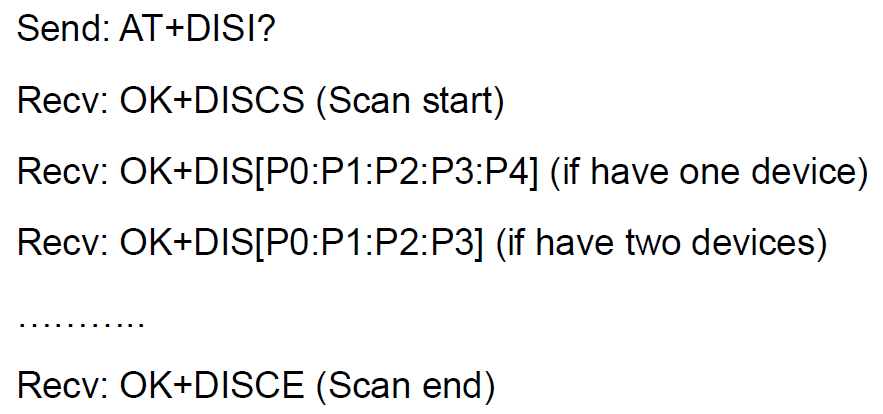
\includegraphics[scale=0.7]{Bilder/disi_command.PNG} 
\caption[Rückgabe des AR+DISI? Befehls]{P0: Factory ID (8 Byte); P1: IBeacon UUID (32 Byte); P2: Major-, Minorvalue, Measured Power (10 Byte); P3: Media-Access-Control-Adresse MAC (12 Byte); P4: RSSI (4 Byte) \cite{hm11Datasheet}}
\label{fig:disiCommand}
\end{figure}
Dafür wird vom MCU jeder char, rsp. jedes Byte vom Datenbuffer ausgelesen und verwertet. Es wird zuerst nach einer UUID eines IBeacons gefiltert und dann die ersten drei Zahlen in einen Integer gecastet. Anschließend soll das Majorvalue\footnote{Major- und Minorvalues dienen hauptsächlich zur zusätzlichen Identifikation eines IBeacons}, welches einen bestimmten, selbst wählbaren Wert hat, abgeglichen werden, damit nur die IBeacons berücksichtig werden, die relevant sind. Ist der empfangene RSSI-Wert grösser als -90dbm, wird der IBeacon eingespeichert. Dies wird mit jedem empfangenen IBeacon wiederholt und immer die RSSI-Werte miteinander verglichen, wobei dann der IBeacon mit dem grösseren RSSI-Wert ins System gespeichert und als Returnvalue von der scan() Funktion zurückgegeben wird.
\section{Validierung}
Für die Validierung wurden zwei IBeacons mit Androidhandys simuliert (Beacon Simulator App). Dafür wurden diese mit einer Distanz von ungefähr $6m$ zueinander auf einer Höhe von ca. $2m$ platziert. Um die detektierten IBeacons direkt auszuwerten, wurde die UUID auf einen Emulator (Putty) über eine serielle Schnittstelle (USB Typ micro B) herausgeschrieben. Somit konnte verifiziert werden, dass der vom Dojo detektierte IBeacon auch der sich am Dojo nächsten befindliche IBeacon war. 
\\[0.5cm]
Eine definitive Distanzbestimmung zwischen dem IBeacon und dem Dojo ist schwierig, da die Sendeleistung der simulierten IBeacons etwas schwanken. Auch die Auslegung des Raumes, sowie die Einrichtung kann das Signal abschwächen, was direkten Einfluss auf die Erkennungsdistanz hat. Es kann aber festgehalten werden, dass ein IBeacon in einem Umkreis von $3m$ garantiert erkennt wird, solange sich keine Gegenstände unmittelbar zwischen den beiden Objekten befinden.